\documentclass[12pt,a4paper]{article}


\setlength{\textwidth}{165mm}
\setlength{\textheight}{240mm}
\setlength{\parindent}{0mm} % S{\aa} meget rykkes ind efter afsnit
\setlength{\parskip}{\parsep}
\setlength{\headheight}{0mm}
\setlength{\headsep}{0mm}
\setlength{\hoffset}{-2.5mm}
\setlength{\voffset}{0mm}
\setlength{\footskip}{15mm}
\setlength{\oddsidemargin}{0mm}
\setlength{\topmargin}{0mm}
\setlength{\evensidemargin}{0mm}

%til tables!
\usepackage[T1]{fontenc}
\usepackage[utf8]{inputenc}
% jubiii
\usepackage{tabularx,ragged2e,booktabs,caption}
\usepackage{algorithm,algpseudocode}
\usepackage[T1]{fontenc}
\usepackage[all]{xy}
\usepackage{graphicx}    % For grafik (billederfiler)
\usepackage[T1]{fontenc} % For at blande \textsc{} med \textbf{}
\usepackage[utf8]{inputenc}
\usepackage{amsfonts,amsmath,amssymb}
\usepackage{eucal}
\usepackage[danish]{babel}
\usepackage{enumerate}  
\usepackage{hyperref}
\usepackage{url}
\usepackage{array}
\usepackage{mathptmx}
\usepackage{amsmath}
\usepackage{multirow}
\usepackage[dvipsnames,usenames]{color}
\usepackage{tabularx,colortbl,xcolor}

\setlength{\textwidth}{165mm}
\setlength{\textheight}{240mm}
\setlength{\parindent}{0mm} % S{\aa} meget rykkes ind efter afsnit
\setlength{\parskip}{\parsep}
\setlength{\headheight}{0mm}
\setlength{\headsep}{0mm}
\setlength{\hoffset}{-2.5mm}
\setlength{\voffset}{0mm}
\setlength{\footskip}{15mm}
\setlength{\oddsidemargin}{0mm}
\setlength{\topmargin}{0mm}
\setlength{\evensidemargin}{0mm}

%til tables!
\usepackage[T1]{fontenc}
\usepackage[utf8]{inputenc}
% jubiii
\usepackage{tabularx,ragged2e,booktabs,caption}
\usepackage{float}
\usepackage[T1]{fontenc}
\usepackage[all]{xy}
\usepackage{graphicx}    % For grafik (billederfiler)
\usepackage[T1]{fontenc} % For at blande \textsc{} med \textbf{}
\usepackage[utf8]{inputenc}
\usepackage{amsfonts,amsmath,amssymb}
\usepackage{eucal}
\usepackage[danish]{babel}
\usepackage{enumerate}  
\usepackage{hyperref}
\usepackage{url}
\usepackage{array}
\usepackage{mathptmx}
\usepackage{amsmath}
\usepackage{multirow}
\usepackage[dvipsnames,usenames]{color}
\usepackage{tabularx,colortbl,xcolor}

\DeclareSymbolFont{usualmathcal}{OMS}{cmsy}{m}{n}
\DeclareSymbolFontAlphabet{\mathcal}{usualmathcal}

% til tables
\newcolumntype{C}[1]{>{\Centering}m{#1}}
\renewcommand\tabularxcolumn[1]{C{#1}}
% jubiii


\begin{document}
\title{PKSU Delrapport 2}
\maketitle
\begin{center}
Jeppe Schönemann Skov, Rose Sofie Greve, Frederik Leed Henriksen \\ \hfill \\ \hfill \\ 
\end{center}
\newpage
\tableofcontents
\newpage
\section{Abstract}
We are making a website for a small Bed and Breakfast on Isla Margarita, Venezuela. The place is working towards becoming a sustainable and self-sufficient mini-hostel, where guests can enjoy organic greens from the garden.
The frontpage on the website will contain a description of the place and the surrounding area.
The website will contain a simple booking- and online payment system.
The website will have a link with pictures of the houses and surrounding facilities, and a link with information on the different activities taking place at the hostel.
With courtesy to the place working with ecology and sustainability, the layout of the website will be simple and inspired by the colors of nature.
Further, we will make an administration part of the system, from where our costumer can see and edit the bookings. The administrator will also be able to edit the website photos and text descriptions. \\\\
\textbf{Changelog}\\\\
Jeppe Schönemann Skov - JSS\\
Frederik Leed Henriksen - FLH\\
Rose Sofie Greve - RSG\\

\begin{table}[h]
\begin{tabular}{lllll}
\cline{1-4}
\multicolumn{1}{|l|}{Initialer} & \multicolumn{1}{l|}{Dato} & \multicolumn{1}{l|}{Afsnit} & \multicolumn{1}{l|}{Ændring} &  \\ \cline{1-4}
\multicolumn{1}{|l|}{JSS, FLH, RSG}     & \multicolumn{1}{l|}{23.04.15}     & \multicolumn{1}{l|}{Alle}       & \multicolumn{1}{l|}{Release edition 1.0}        &  \\ \cline{1-4}
\multicolumn{1}{|l|}{RSG}     & \multicolumn{1}{l|}{07.05.15}     & \multicolumn{1}{l|}{1, 2}       & \multicolumn{1}{l|}{Stavefejl, mere præcis beskrivelse}        &  \\ \cline{1-4}
\multicolumn{1}{|l|}{RSG}     & \multicolumn{1}{l|}{07.05.15}     & \multicolumn{1}{l|}{3.a}       & \multicolumn{1}{l|}{Krav i stikord, mere uddybende}        &  \\ \cline{1-4}
\multicolumn{1}{|l|}{FLH}     & \multicolumn{1}{l|}{07.05.15}     & \multicolumn{1}{l|}{3.b, 3.c, 3.e}       & \multicolumn{1}{l|}{Omskrivning og ændring i model}        &  \\ \cline{1-4}
\multicolumn{1}{|l|}{JSS}     & \multicolumn{1}{l|}{07.05.15}     & \multicolumn{1}{l|}{3.d}       & \multicolumn{1}{l|}{Opdateret klassediagramet}        &  \\ \cline{1-4}
\multicolumn{1}{|l|}{RSG, JSS}     & \multicolumn{1}{l|}{07.05.15}     & \multicolumn{1}{l|}{3.f}       & \multicolumn{1}{l|}{Kommentarer til firgurer}        &  \\ \cline{1-4}
\multicolumn{1}{|l|}{RSG, JSS}     & \multicolumn{1}{l|}{07.05.15}     & \multicolumn{1}{l|}{6, 7}       & \multicolumn{1}{l|}{Ændring i tekst}        &  \\ \cline{1-4}
\multicolumn{1}{|l|}{RSG}     & \multicolumn{1}{l|}{11.05.15}     & \multicolumn{1}{l|}{4, 5, 7}       & \multicolumn{1}{l|}{Ændring i tekst}        &  \\ \cline{1-4}
\multicolumn{1}{|l|}{FLH}     & \multicolumn{1}{l|}{11.05.15}     & \multicolumn{1}{l|}{6}       & \multicolumn{1}{l|}{Flowchart, skærmbilleder}        &  \\ \cline{1-4}
                           &                           &                             &                              & 
\end{tabular}
\end{table}


\newpage
\section{IT-projektets formål og rammer}
Her følger en beskrivelse af rammerne for vores IT-projekt, baseret på FACTOR-begrebet.
\\\\
Functionality: Skal indeholde et booking- og betalingssystem, hvor administratoren har mulighed for at redigere i bookingerne. Samt sider billeder og information om hostelet. \\

Application domain: Skal administrere bookninger, herunder til- og afmelde folk samt finde kontaktoplysninger på de folk der har oprettet en booking.\\
 
Conditions: Udvikling og endeligt brug af systemet skal være minded på, at dem der skal betjene det, ikke har stor teknisk erfaring. Vi skal derfor udvikle minded på, at de tekniske detaljer ikke er deres fokus.\\

Technology: Systemet skal både udvikles og kunne betjenes på en billig pc med internet. Grundet hyppige strømsvigt skal databasen ligge på en webserver. \\

Objects: Personer der ønsker at booke værelse. Administrering af bookinger og websiden.\\

Responsibility: Systemet skal løse administrative problematikker i henhold til at holde styr på kontaktoplysninger af kunder. Holde styr på hvilke værelser der er ledige, og hvornår disse er ledige. Systemet skal også reklamere for hostel'et.\\
\newpage
\section{Kravspecifikationer for IT-løsningen}
\subsection{a}
\textbf{Funktionelle krav:} \\
- Side med bookingsystem der giver brugeren mulighed for at booke senge\\
- Administrativ side der giver vores kunde mulighed for at redigere i bookinger, tekst og billeder på brugersiden\\
- Betaingssystem\\\\
       \textbf{Ikke-funktionelle krav:} \\
- Simpelt system, som kan benyttes af folk uden særlig teknisk erfaring\\
- Side med information om stedet\\
- Side med billedegalleri\\
- Side med kontaktinformation\\
- Layout der afspejler hostelets stil og holdning til miljøet. \\\\
      \textbf{Begrænsninger:} \\
	Siden skal kunne vises på en billig computer og uden hurtigt internet til rådighed. Databasen med bookinger skal ligge på en webserver, da strømsvigt er hyppige i området.
\subsection{b}
\begin{figure}[H]
\centering
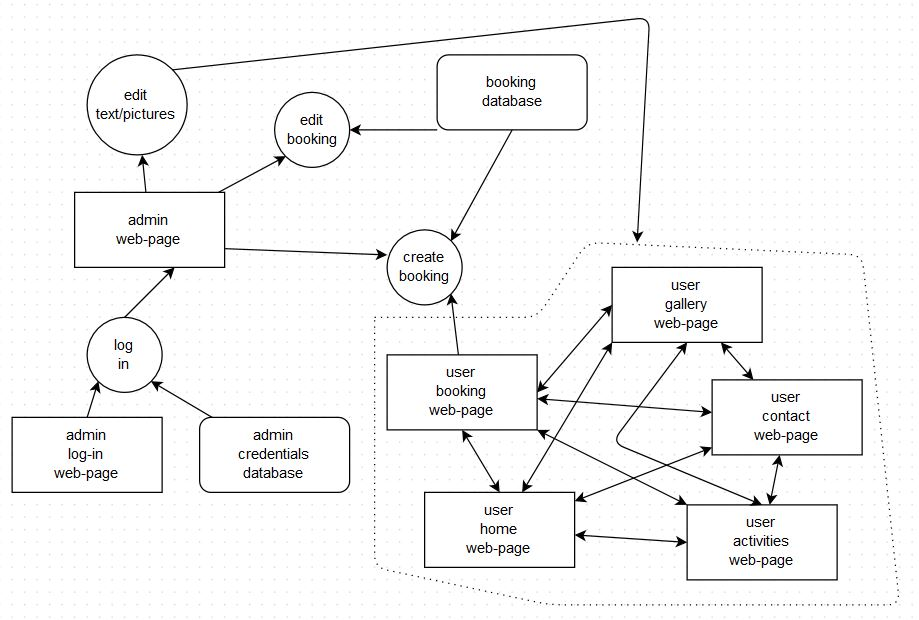
\includegraphics[scale=0.7]{usecasemodelV2.jpg}
\caption{Use Case model}
\end{figure}
Figur 1 illustrerer brugersiderne gallery, activities, home, contact og booking. Brugeren har gennem siden booking mulighed for at booke senge på hostelet. Bookingen bliver gemt i booking databasen. Den administrasive side kræver login. Der findes en database, der holder styr på logindetaljerne. Fra den administrative side kan kunden se og redigere i bookingerne samt teksten og billederne på de forskellige sider.\\
\subsection{c}

\begin{minipage}{\textwidth}

\captionof{table}{\textbf{Admin log-in}} \label{tab:title}
\begin{tabular}{| p{5cm} p{10cm} |}
\hline use-case-name & Admin log-in \\
\hline participating actors & administratoren \\
\hline flow of events & \begin{enumerate}
\item administratoren intaster sit log-in på admin log-in siden og trykker på log-in knappen
\item admindatabasen bliver spurgt om de indsendte oplysninger er rigtige.
\item hvis der findes et match, bliver man videreført til admin-siden. Hvis ikke får man en fejlmeddelelse.
\end{enumerate} \\
\hline Entry conditions & ingen \\
\hline Exit conditions & ingen \\
\hline
\end{tabular}

\end{minipage}

\bigskip

\begin{minipage}{\textwidth}

\captionof{table}{\textbf{Admin slet booking}} \label{tab:title}
\begin{tabular}{| p{5cm} p{10cm} |}
\hline use-case-name & Admin slet booking \\
\hline participating actors & administratoren \\
\hline flow of events & \begin{enumerate}
\item administratoren trykker på slet knappen i tabellen ud for bookingen 
\item ændringen bliver sendt til databasen og bookingen slettes
\item tabellen opdateres og bookingen er slettet og vises ikke mere
\end{enumerate} \\
\hline Entry conditions & admin log-in \\
\hline Exit conditions & ingen \\
\hline
\end{tabular}

\end{minipage}
	
\bigskip

\begin{minipage}{\textwidth}

\captionof{table}{\textbf{kunde booking}} \label{tab:title}
\begin{tabular}{| p{5cm} p{10cm} |}
\hline use-case-name & kunde booking \\
\hline participating actors & kunden \\
\hline flow of events & \begin{enumerate}
\item kunden indtaster sine ønskede booking datoer og kontaktinformationer 
\item kunden trykker på booking knappen og booking informationerne bliver tjekket for at verificere om bookingen ikke overlapper med andre bookinger
\item hvis der ikke er nogen overlab, bliver bookingen oprettet og kunden bliver videresendt til "home" siden. Hvis der er overlab får kunden en fejlmeddelelse
\end{enumerate} \\
\hline Entry conditions & at kunden befinder sig på bookingsiden \\
\hline Exit conditions & ingen \\
\hline
\end{tabular}

\end{minipage}	
	
\subsection{d}
\begin{figure}[H]
\centering
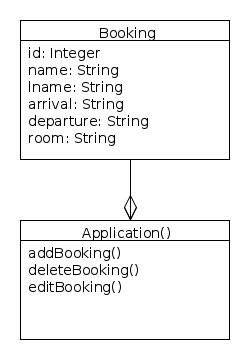
\includegraphics[scale=0.6]{BookingSystem.jpg}
\caption{Booking system - UML}
\end{figure}
Figur 2 illustrerer et klassediagram over vores bookingsystem. Application() tilføjer, redigerer og sletter bookinger fra bookingdatabasen. Booking definerer hvilke parametre en booking skal indeholde.
\subsection{e}

\begin{minipage}{\textwidth}

\captionof{table}{\textbf{Boundary}} \label{tab:title}
\begin{tabular}{| p{5cm} | p{10cm} |}
\hline Admin log-in side & web-siden for administratoren som benyttes til at verificere at personen er administrator \\
\hline kunde booking web-side & her har kunden adgang til at oprette en booking samt navigering til de andre kunde sider \\
\hline kunde "home" web-side & her kan kunden navigere til de andre sider \\
\hline kunde galleri web-side & her kan kunden navigere til de andre sider \\
\hline kunde kontakt web-side & her kan kunden navigere til de andre sider \\
\hline kunde aktiviteter web-side & her kan kunden navigere til de andre sider \\
\hline
\end{tabular}

\end{minipage}

\bigskip

\begin{minipage}{\textwidth}

\captionof{table}{\textbf{Control}} \label{tab:title}
\begin{tabular}{| p{5cm} | p{10cm} |}
\hline admin log-in \newline verificeringsknappen & facillitere forespørgslen mellem admin log-in siden og admin databasen, hvis personen er en admin, bliver vedkommende sendt videre til admin siden. hvis ikke, sker der ikke noget.\\
\hline opret booking knap & søger databasen for overlap i dato. Hvis der ikke er sådanne konflikter skabes en booking med de givne informationer i databasen, hvis der er en konflikt vises en passende fejlmeddelelse \\
\hline fjern booking knap & fjerner en oprettet booking fra databasen \\
\hline rediger web-sider & redigere kundesidernes indhold i forhold til billeder og tekst ( vi ved endnu ikke hvordan dette skal implementeres) \\
\hline "home" link & sender kunden til "home" web-page \\
\hline booking link & sender kunden til booking web-page \\
\hline galleri link & sender kunden til galleri web-page \\
\hline kontakt link & sender kunden til kontakt web-page \\
\hline aktiviteter link & sender kunden til aktiviteter web-page \\
\hline
\end{tabular}

\end{minipage}

\bigskip

\begin{minipage}{\textwidth}

\captionof{table}{\textbf{Entity}} \label{tab:title}
\begin{tabular}{| p{5cm} | p{10cm} |}
\hline Admin databasen & indeholder oplysninger om hvilke brugere der eksistere i systemet \\
\hline administrator siden & Her har administrator mulighed for at tilse aktuelle bookninger og rette i databasen \\
\hline booking database & indeholder alle bookinger på siden \\
\hline
\end{tabular}

\end{minipage}

\subsection{f}

\begin{figure}[H]
\centering
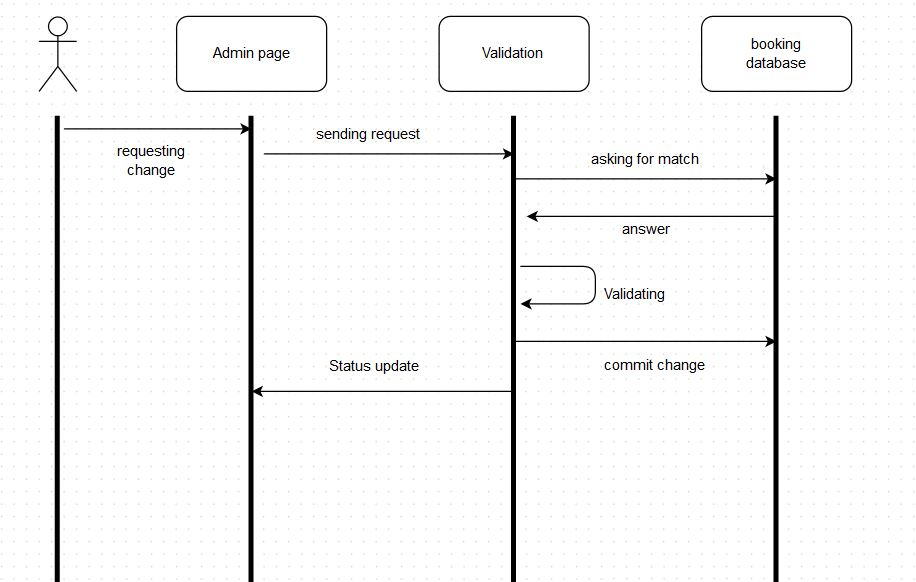
\includegraphics[scale=0.6]{adminInteraction.jpg}
\caption{Admin Interaction}
\end{figure}
Figur 4 illustrerer interaktionen mellem den administrative side og bookingdatabasen.\\
\begin{figure}[H]
\centering
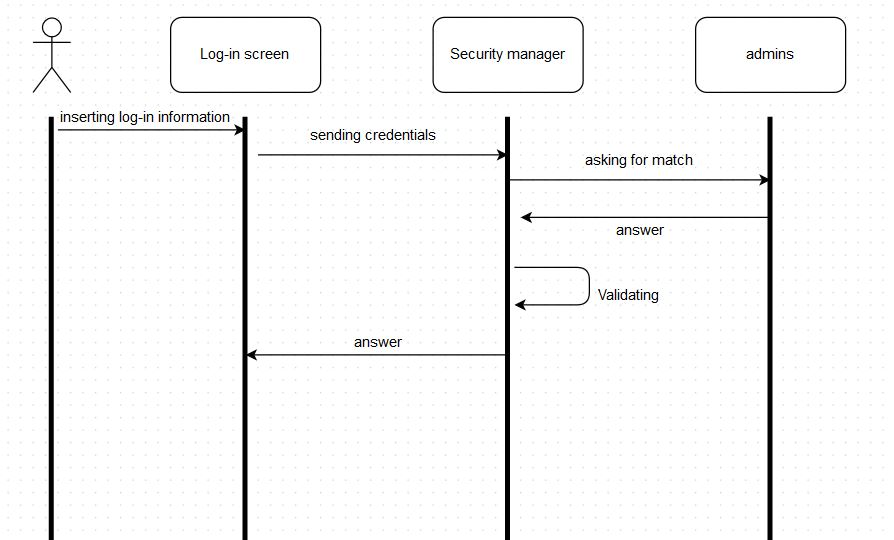
\includegraphics[scale=0.6]{adminLog-in.jpg}
\caption{Admin log-in}
\end{figure}
Figur 5 illusterer valideringprocessen ved login på den administrative side.\\
\begin{figure}[H]
\centering
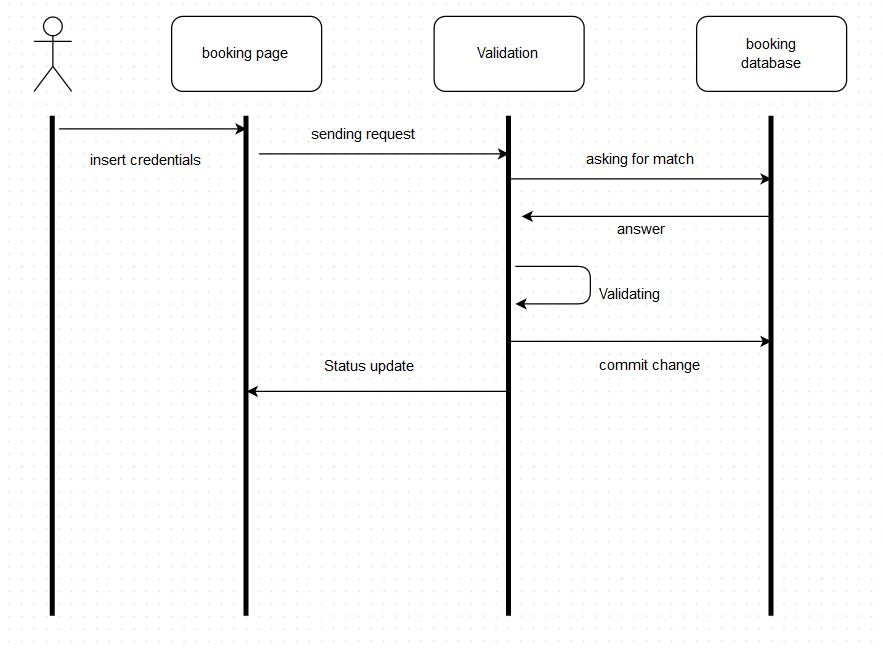
\includegraphics[scale=0.6]{customerLog-in.jpg}
\caption{Customer Interaction}
\end{figure}
Firgur 6 illustrerer processen når en bruger forsøger at oprette en booking.
\newpage
\section{Systemdesign sammenfatning}
\textbf{Systemet som det er nu:}
Vi har benyttet Play! frameworket til at lave en meget fin prototype at systemet.
Det er nu muligt at navigere mellem alle de forskellige sider, på hjemmesiden. Vi har fået implementeret en billede-slider på siden \textit{Gallery}, som præsenterer billeder af stedet i et diasshow. På siden \textit{Contact} har vi implementeret et google-maps kort, der viser hostelets beliggenhed. Bookingsystemet er også blevet konstrueret, og det er nu muligt at tilføje en booking fra bruger-siden, samt tilføje og slette bookinger fra admin-siden. Bookingerne gemmes i en database.    

\textbf{De væsentligste mangler:}
Vi mangler en funktion der gør det muligt for administratoren at ændre en booking. Desuden mangler vi stadig at lave et login-system til admin-siden.\\
Vi skal også gøre det muligt for kunden, selv at bestemme hvilke billeder der fremvises samt redigere i teksten på de forskellige sider. Endeligt mangler vi at koble bookingsystemet til et betalingssystem.
\section{Program- og systemtest}
Indtil videre har vi kun testet vores system visuelt, og alt virker som vi ønsker. Vi har endnu ikke sat begrænsninger på bookingsystemet, sådan at to bookinger ikke overlapper hinanden. Planen er at lave en test-klasse, der kan teste bookingsystemet med Junit.

\section{Brugergrænseflade og interaktonsdesign}
Fra menu bjælken kan brugeren navigerer sig rundt på hele hjemmesiden. Menubjælken vil være tilstede lige meget hvor brugeren befinder sig henne på siden.
Hjemmesiden benytter sig af konceptet REST, hvilket vil sige at siderne er uafhængige, og ingen relationer har til hinanden.

\section{Projektsamarbejdet}
Internt i gruppen arbejder vi godt sammen. For nogle uger siden besluttede vi os for at sætte mandag og torsdag af til at arbejde på projektet. Siden da er vi nået rigtig langt med systemet. 

Vi har indtil videre haft tre møder med kunden. Møderne foregår over Skype, da kunden bor i Venezuela. På trods af at afstanden kan være upraktisk, er kunden fleksibel med dato for møder, da vi blot mødes over Skype.

Under møderne tager vi referat i form af stikord, og dokumenterer de aftalte ændringer i projektaftalen og projektplanen, i rapporten. 

Under første møde d. 19. februar 2015 fik vi lavet en projektaftale med kunden.\\
Under andet møde d. 10. marts 2015 snakkede vi detaljer ift. bookingsystemet.\\
Under tredje møde d. 15. april 2015 snakkede vi om valg af betalingssystem, samt om hvilke dele af projektet kunden helst så os nedprioritere i tilfælde af tidspres.

Vi har endnu ikke en fast dato for næste møde, da kunden som sagt er fleksibel, og vi derfor kan kontakte hende, når vi har brug for at diskutere projektet.
\newpage
\section{Litteraturreview}
\subsection{Designing for usability}
Denne artikel beskriver tre design principper, som Gould og Lewis mener er vigtige, men selv om de måske virker indlysende, bliver de ofte forsømt af udviklerne af flere årsager. Udviklerne undervurderer eller misforstår simpelthen nogle gange disse ”simple” principper. De tre principper: 

Fokus på målgruppe og opgaver. 
Hvor designeren må vide hvem målgruppen er og være i direkte kontakt med udviklerne, for at de kan analysere og studere målgruppens adfærd i stedet for at bare læse eller høre om dem. 

Simulation og prototype.
Målgruppen skal afprøve prototypen, hvor deres reaktion og ydeevne på systemet analyseres og observeres.

Test og omstrukturer.
Det sidste princip dækker over test af systemet og de fejl, som bliver fundet, skal rettes, og hvis det bliver nødvendigt, skal programmet omstruktureres og testes forfra.

Derefter uddyber de principperne, og forklarer, hvordan de kan anvendes i starten af design fasen efterfulgt af en test fase. De slutter deres diskussion ved at præsentere et case studie, hvor de anvender disse principper i et lyd besked system fra IBM.   

Det er svært at argumentere mod vigtigheden af disse principper, som måske virker meget basale, men det kan være meget let undervurdere vigtigheden af disse principper. Object-Oriented Software Engineering Using UML, Patterns, and Java bogen beskriver seks faser, når man udvikler et system.

Krav
Analyse
System Design
Objekt Design
Implementation
Test

Hvor den ligger meget vægt på samarbejde med kunden i form af modeller og grafiske illustration i stedet for at arbejde sammen med målgruppen, som jeg syntes artiklen ligger op til.

I vores projekt hvor vi har til opgave at designe og lave et online sommerhus booking system, forsøger vi at holde en løbende dialog med vores kunde. Vi fik først og fremmest nogle krav fra kunden, som vi skal overholde, men da de fleste var kommet på plads, og vi havde en nogenlunde idé om, hvad vi egentlig skulle lave i vores projekt. Dernæst har vi planer om at lave vores prototype af hjemmeside færdig, og derefter have et interview med vores kunde, for at se om de er tilfredse, eller om de har nogle ændringer. Efter det har vi planer om at nå ud til målgruppen med prototypen og høre deres mening om systemet, og om det er brugervenligt.
\subsection{A rational design process}
A Rational Design Process forklarer om hvad den rationelle design process er, og hvorfor det er så svært at lave en rationel struktur på sit projekt.

Kort sagt går et rationelt design ud på, at man stiller nogle helt præcise krav op for sit projekt. At man opdeler projektet i mindre og mindre detaljerede dele, indtil man har en fuldstændig plan for, hvordan man vil udføre sit projekt. Og at man dokumenterer alle beslutninger og ændringer, man foretager sig løbende.

Det er dog sjældent, at programmørens valg i den initielle designfase er særligt rationelle. Dette er der flere årsager til. Som vi selv har kunne mærke i vores projekt, vil der i starten ofte være uklarhed omkring, præcis hvad systemet skal kunne. Mange detaljer dukker altid op løbende under design- og programmeringsprocessen, og det er derfor ikke muligt fra start af at lave en nøjagtig plan. Selv hvis det var muligt at kende til alle projektets detaljer på en gang, vil det simpelthen være for stor en mundfuld information, til at det er muligt for den menneskelige hjerne at lave et endeligt softwaredesign. Der sker ofte ændringer i, hvad systemet skal indebære. Disse ændringer har ofte betydning for designet, og man ville altså alligevel ende med et andet design end det første “rationelle design” man havde konstrueret. Endeligt sker det tit, at man skal viderearbejde allerede eksisterende software, som allerede har et design. Et rationelt design kan også udelukke muligheden for nye og anderledes ideer til design, inspireret af andre projekter, hvis design ikke nødvendigvis er særligt rationelt, men som på en anden måde virker optimalt for ens projekt.

På trods af alle disse stopklodser for en rationel design process er der også mange positive sider ved at forsøge at lave et rationelt design. Der researches derfor en del i en struktureret ”opskrift” på software design.
Ligger man tid og kræfter i at få lavet et godt solidt design, før man går i gang med at kode, bliver man tvunget til at reflektere over hele projektet, og tage stilling til hvilke udfordringer man måske støder på. Dette vil spare én tid i den anden ende.

Vi er opsatte på at forsøge os med at lave en detaljeret projektplan, da vi efterhånden begynder at forstå nødvendigheden af at have et godt overblik over det system, vi arbejder på. Vi vil også få lavet noget ordentlig dokumentation, for de valg vi tager, så vi på senere tidspunkter kan finde svar på, hvorfor vi valgte at gøre som vi gjorde. 
Dog er der mange ting, vi har svært ved at forestille os på dette tidlige stadie, især fordi at ingen af os har nogen programmeringserfaring. Det gør det f.eks. svært for os at vide, hvordan vi egentlig skal inddele projektet i moduler/subsystems, samt hvor lang tid hver del af projektet vil tage.

Vi anser opskriften på hvordan man laver et rationelt design som en slags guide og inspiration til, hvordan man kan gribe et projekt an. I forsøget på at følge opskriften på det rationelle design vil man eksempelvis lægge et større arbejde i at finde de små detaljer og risici ved projektet så tidligt som muligt og dermed undgå for meget back-tracking.
Ved efterfølgende at skrive sin dokumentation og projektplan som hvis man havde fulgt det perfekte design, altså ”fake” den ideelle process, bliver man stadig tvunget til at være mere reflekteret og forberedt, og gør dermed projektet og ens egen arbejde mere struktureret. 
\end{document}